\documentclass[10pt,a4paper,twoside,twocolumn]{article}%ustalasz jaki typ dokumentu i właściwości

\usepackage[polish]{babel} % ustawianie języka polskiego
\usepackage[colorlinks=false,linkcolor=green,urlcolor=green,citecolor=green]{hyperref}%hiperłącza ogólnego rodzaju
\hypersetup{pdftitle=Sprawozdanie SSR}

\usepackage{pdfpages} % importowanie plików z pdfa
\usepackage{amsmath} % do wstawiania macierz itp
\usepackage{graphicx} % wstawianie zdjęć
% \usepackage[utf8]{inputenc} % niepotrzebne bo lualatex
\usepackage[T1]{fontenc} % niepotrzebne bo lualatex
\usepackage[left=2cm,right=2cm,top=2cm,bottom=2cm,
columnsep=1.5cm % odstęp między kolumnami
]{geometry}%marginesy

\usepackage{listings} % punktowanie
% \usepackage{indentfirst} % dawanie akapitu na początku
\usepackage{caption} % podpisy
\usepackage{subcaption} % podpisy do subfigure
\usepackage{siunitx} % jednostki si
\usepackage{minted} % ładne kody naprzyklad matlaba
\setminted{linenos=true,frame=single,breaklines=true,breaksymbolleft=,style=vs}

\usepackage{textcase}

\usepackage[polish,nameinlink]{cleveref} % dobre prefiksy przed etykietą i język
\usepackage{cprotect}

\usepackage{fontspec}
% \setmainfont[Ligatures=TeX]{Georgia}
% \setsansfont[Ligatures=TeX]{Arial}
\usepackage{parskip} % usunięcie tab na początku akapitu
\usepackage{newfloat} % aby można było ładnie wstawić elementy typu zdjecie, kod itp

%%% rysowanie wykresów %%% ale w ciul to trudne więc app.diagrams.net
\usepackage{tikz}
\usetikzlibrary{shapes.geometric, arrows, positioning}

% % % SVG import
\usepackage{svg}
\usepackage{import}
\usepackage{xifthen}
\usepackage{transparent}

% \usepackage{mdframed} % ramki
\usepackage[framemethod=TikZ]{mdframed}
\mdfsetup{%
middlelinecolor=red,
middlelinewidth=1pt,
   backgroundcolor=gray!20,
   roundcorner=10pt}

\usepackage{enumitem} % podpunkty customowe

\usepackage{pgfplots}[compat=1.18] % wykresy


%%%%%%%%%%%%%% koniec pakietów %%%%%%%%%%%%%%%%%%%%%%%%%%%

\boldmath%pogrubiona matma

\title{Fajny ten tytuł}%tytuł
\date{\today}%%data
\author{Janusz Chmaruk}%autor
\setcounter{secnumdepth}{3}%głębokość liczenia roździałów

% PRZYKŁAD LICZNIKA ZADAŃ
\newcounter{zadanie}
\newenvironment{zadanie}[1][]{
   \refstepcounter{zadanie}
   \subsection*{Zadanie \thezadanie#1}
   \addcontentsline{toc}{subsection}{Zadanie \thezadanie#1} % dodanie do spisu treści
}{}

% PRZYKŁAD LICZNIKA ROZWIĄZAŃ
\newcounter{rozwiazanie}
\newenvironment{rozwiazanie}[1][]{
   \refstepcounter{rozwiazanie}
   \subsection*{Rozwiazanie zadania \therozwiazanie#1}
   \addcontentsline{toc}{subsection}{Rozwiazanie zadania \therozwiazanie#1} % dodanie do spisu treści
}{}


% DŁUGIE LISTINGI
\newenvironment{longlisting}{\captionsetup{type=listing}}{}

\newcounter{licznikFigure}
\newcommand{\CC}{\refstepcounter{licznikFigure}\caption*{figure \thelicznikFigure}}


%%%%%%%%%%%%%%%%%%%%%%%%%%%%%%%%%%%%%%%%%%%%%%%%%%%%%%%%%%%%%%%
%%%%%%%%%%%%%%%%%%%%%%%%%%%%%%%%%%%%%%%%%%%%%%%%%%%%%%%%%%%%%%%
%%%%%%% TU SIE ZACZYNA PISANIE PLIKU %%%%%%%%%%%%%%%%%%%%%%%%%%
%%%%%%%%%%%%%%%%%%%%%%%%%%%%%%%%%%%%%%%%%%%%%%%%%%%%%%%%%%%%%%%
%%%%%%%%%%%%%%%%%%%%%%%%%%%%%%%%%%%%%%%%%%%%%%%%%%%%%%%%%%%%%%%

\begin{document}%zaczyna się dokument

% Numer rysynku


\null%
\includepdf[pages={1}]{Szablon_Projektu.pdf}
\clearpage%następna strona ogółem

\tableofcontents%spis treści
% \clearpage

\section{Cel ćwiczenia}%sekcja
Celem ćwiczenia jest przybliżenie możliwości wykorzystywania biblioteki Image Processing Toolbox (IPT) do przetwarzania i analizy informacji o barwie zawartej w obrazie cyfrowym. Zakres laboratorium obejmuje: konwertowanie obrazów cyfrowych do innej przestrzeni barw (opisu w rożnych modelach barwnych), pseudokolorowanie, praktyczne wykorzystanie wybranych metod i technik analizy barwnej obrazów cyfrowych.


\section{Kod}
\begin{longlisting}
    \inputminted{matlab}{kod/PSIO3x.m}
\end{longlisting}


Pierwsza część kodu dotyczy wyświetlania rozkładu składowych barw RGB we współrzędnych 3D dla obrazu dog.jpg. Początkowo, kod wczytuje obraz i wyodrębnia składowe czerwony (R), zielony (G) i niebieski (B) do osobnych zmiennych. Następnie, tworzy mapy kolorów dla każdej składowej barwy. Wartość nasycenia Z jest następnie używana do redukcji nasycenia dla każdej składowej barwy, co skutkuje obrazami z zredukowanym nasyceniem dla składowych R, G, i B\@. Te obrazy są następnie wyświetlane jako wykresy przestrzenne. 

W drugiej części kodu, obraz RGB jest konwertowany do trzech różnych reprezentacji barwnych: HSV, Lab, i YCbCr. Te konwersje są użyteczne, ponieważ różne modele barwne mogą lepiej reprezentować pewne aspekty obrazu, takie jak percepcyjna jasność, nasycenie lub odcień. Wynikowe obrazy są następnie wyświetlane. 

Trzecia część kodu obejmuje kilka operacji na obrazie barwnym. Obraz jest najpierw konwertowany do obrazu w odcieniach szarości. Następnie, jest tworzony profil barwny RGB dla wybranego fragmentu obrazu. Wybrany kanał barwny jest modyfikowany (w tym przypadku, poprzez dodanie wartości do kanału czerwonego), a następnie obrazy są skalowane z powrotem do obrazu RGB i wyświetlane. Kolejnym krokiem jest pseudokolorowanie obrazu dla dwóch różnych liczby kolorów (64 i 255), przy użyciu dwóch różnych map kolorów (parula i jet). Na końcu, z obrazu wyodrębniany jest wybrany kolor (w tym przypadku czerwony). 

Czwarta część kodu skupia się na modyfikacji kontrastu obrazu. Zaczyna się od konwersji obrazu do obrazu w odcieniach szarości. Następnie, obraz jest wyświetlany przed regulacją kontrastu. Kontrast jest regulowany dla różnych wartości parametrów za pomocą funkcji imadjust. Na końcu, obrazy po regulacji kontrastu są wyświetlane.

\section{Wyniki}

\begin{figure}[H]
    \centering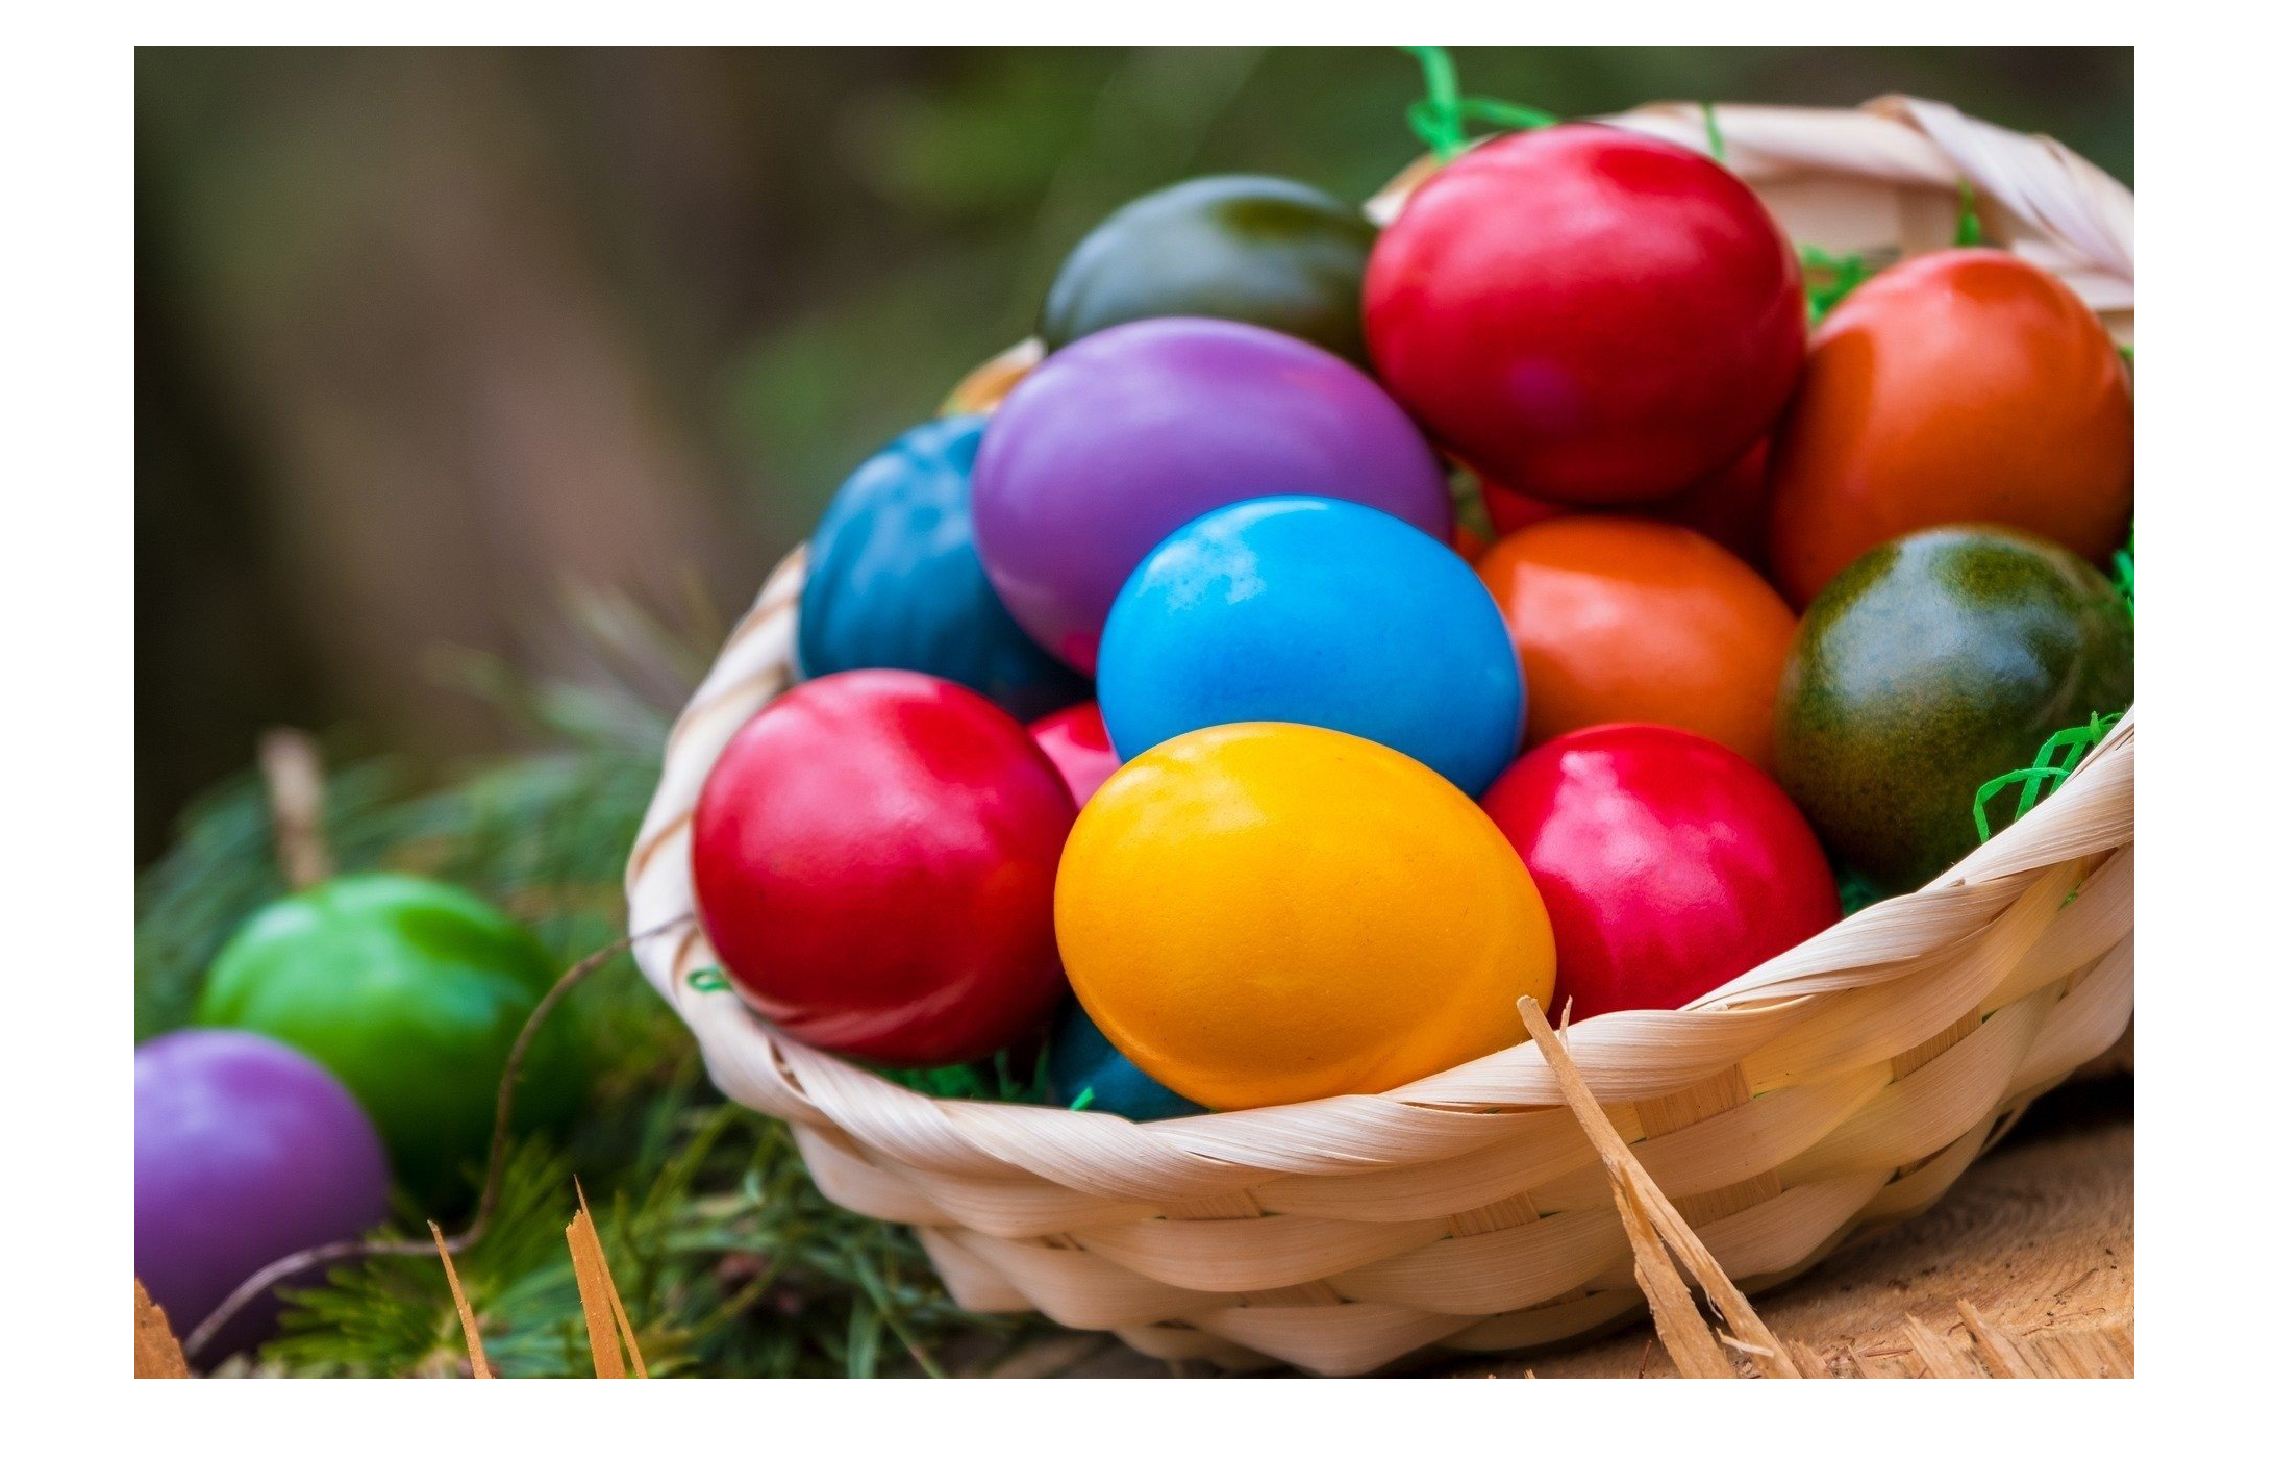
\includegraphics[width=1\linewidth]{kod/my_figure1.pdf}
    \CC\label{fig:my_figure1.pdf}
\end{figure}

\begin{figure}[H]\centering\includegraphics[width=0.9\linewidth]{kod/my_figure2.pdf}\CC\label{fig:my_figure2.pdf}\end{figure}

\begin{figure}[H]\centering\includegraphics[width=0.9\linewidth]{kod/my_figure3.pdf}\CC\label{fig:my_figure3.pdf}\end{figure}

\begin{figure}[H]\centering\includegraphics[width=0.9\linewidth]{kod/my_figure4.pdf}\CC\label{fig:my_figure4.pdf}\end{figure}

\begin{figure}[H]\centering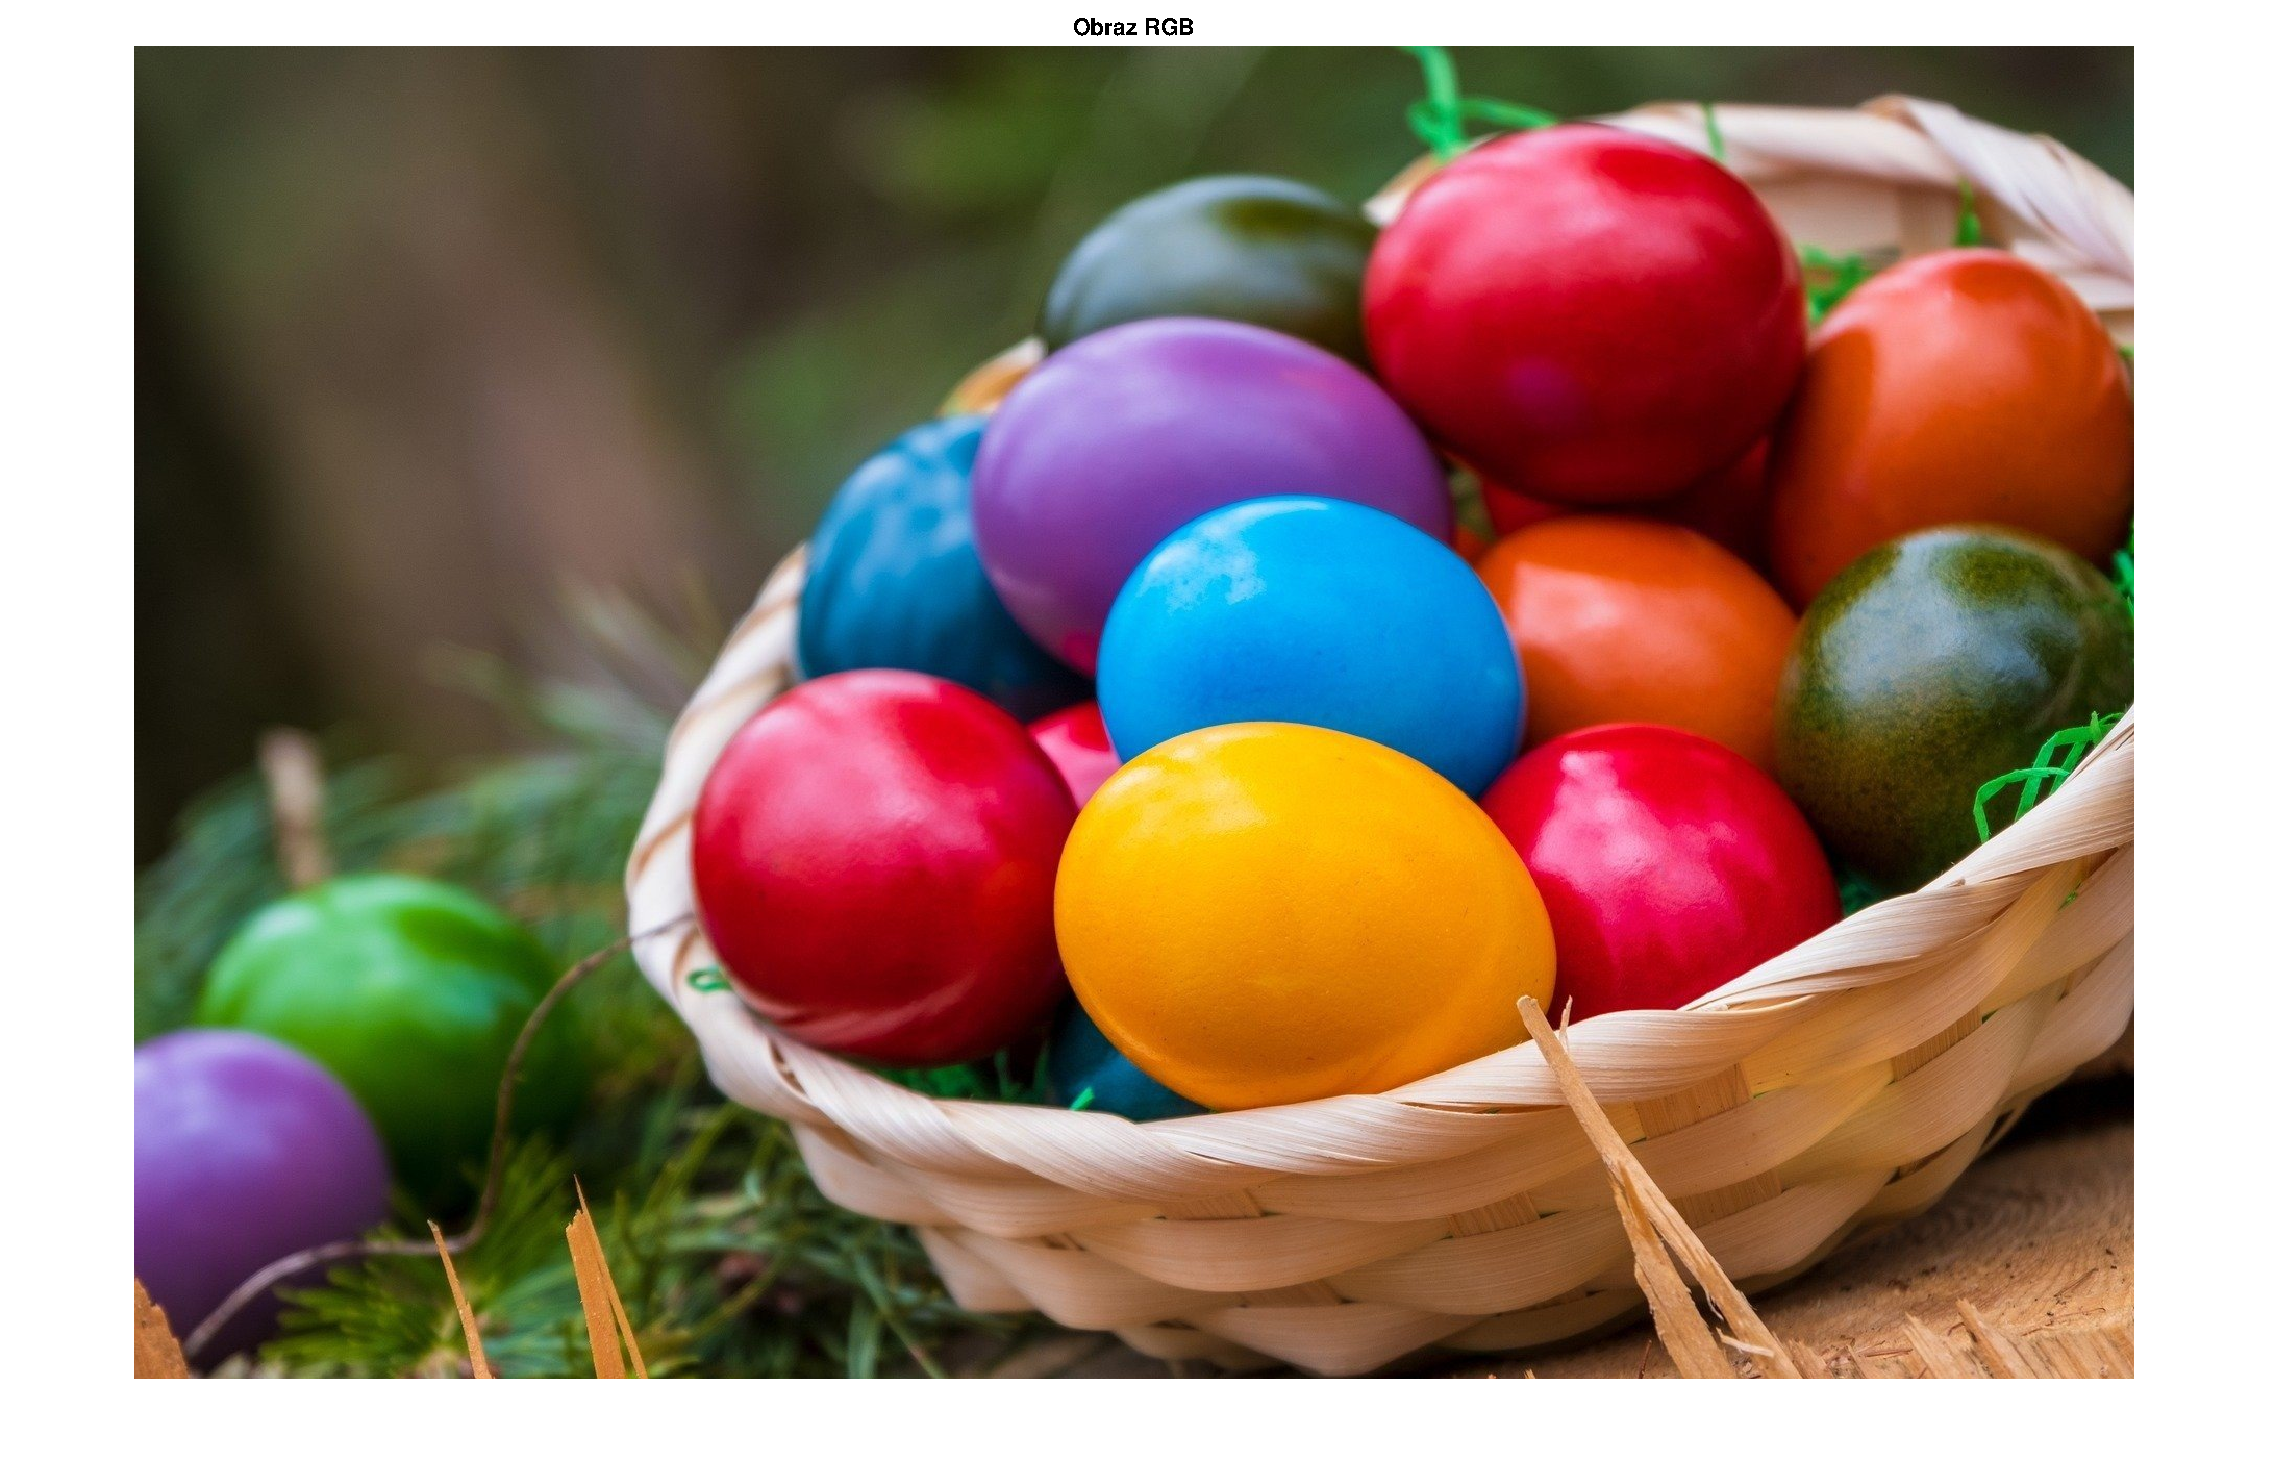
\includegraphics[width=0.9\linewidth]{kod/my_figure5.pdf}\CC\label{fig:my_figure5.pdf}\end{figure}

\begin{figure}[H]\centering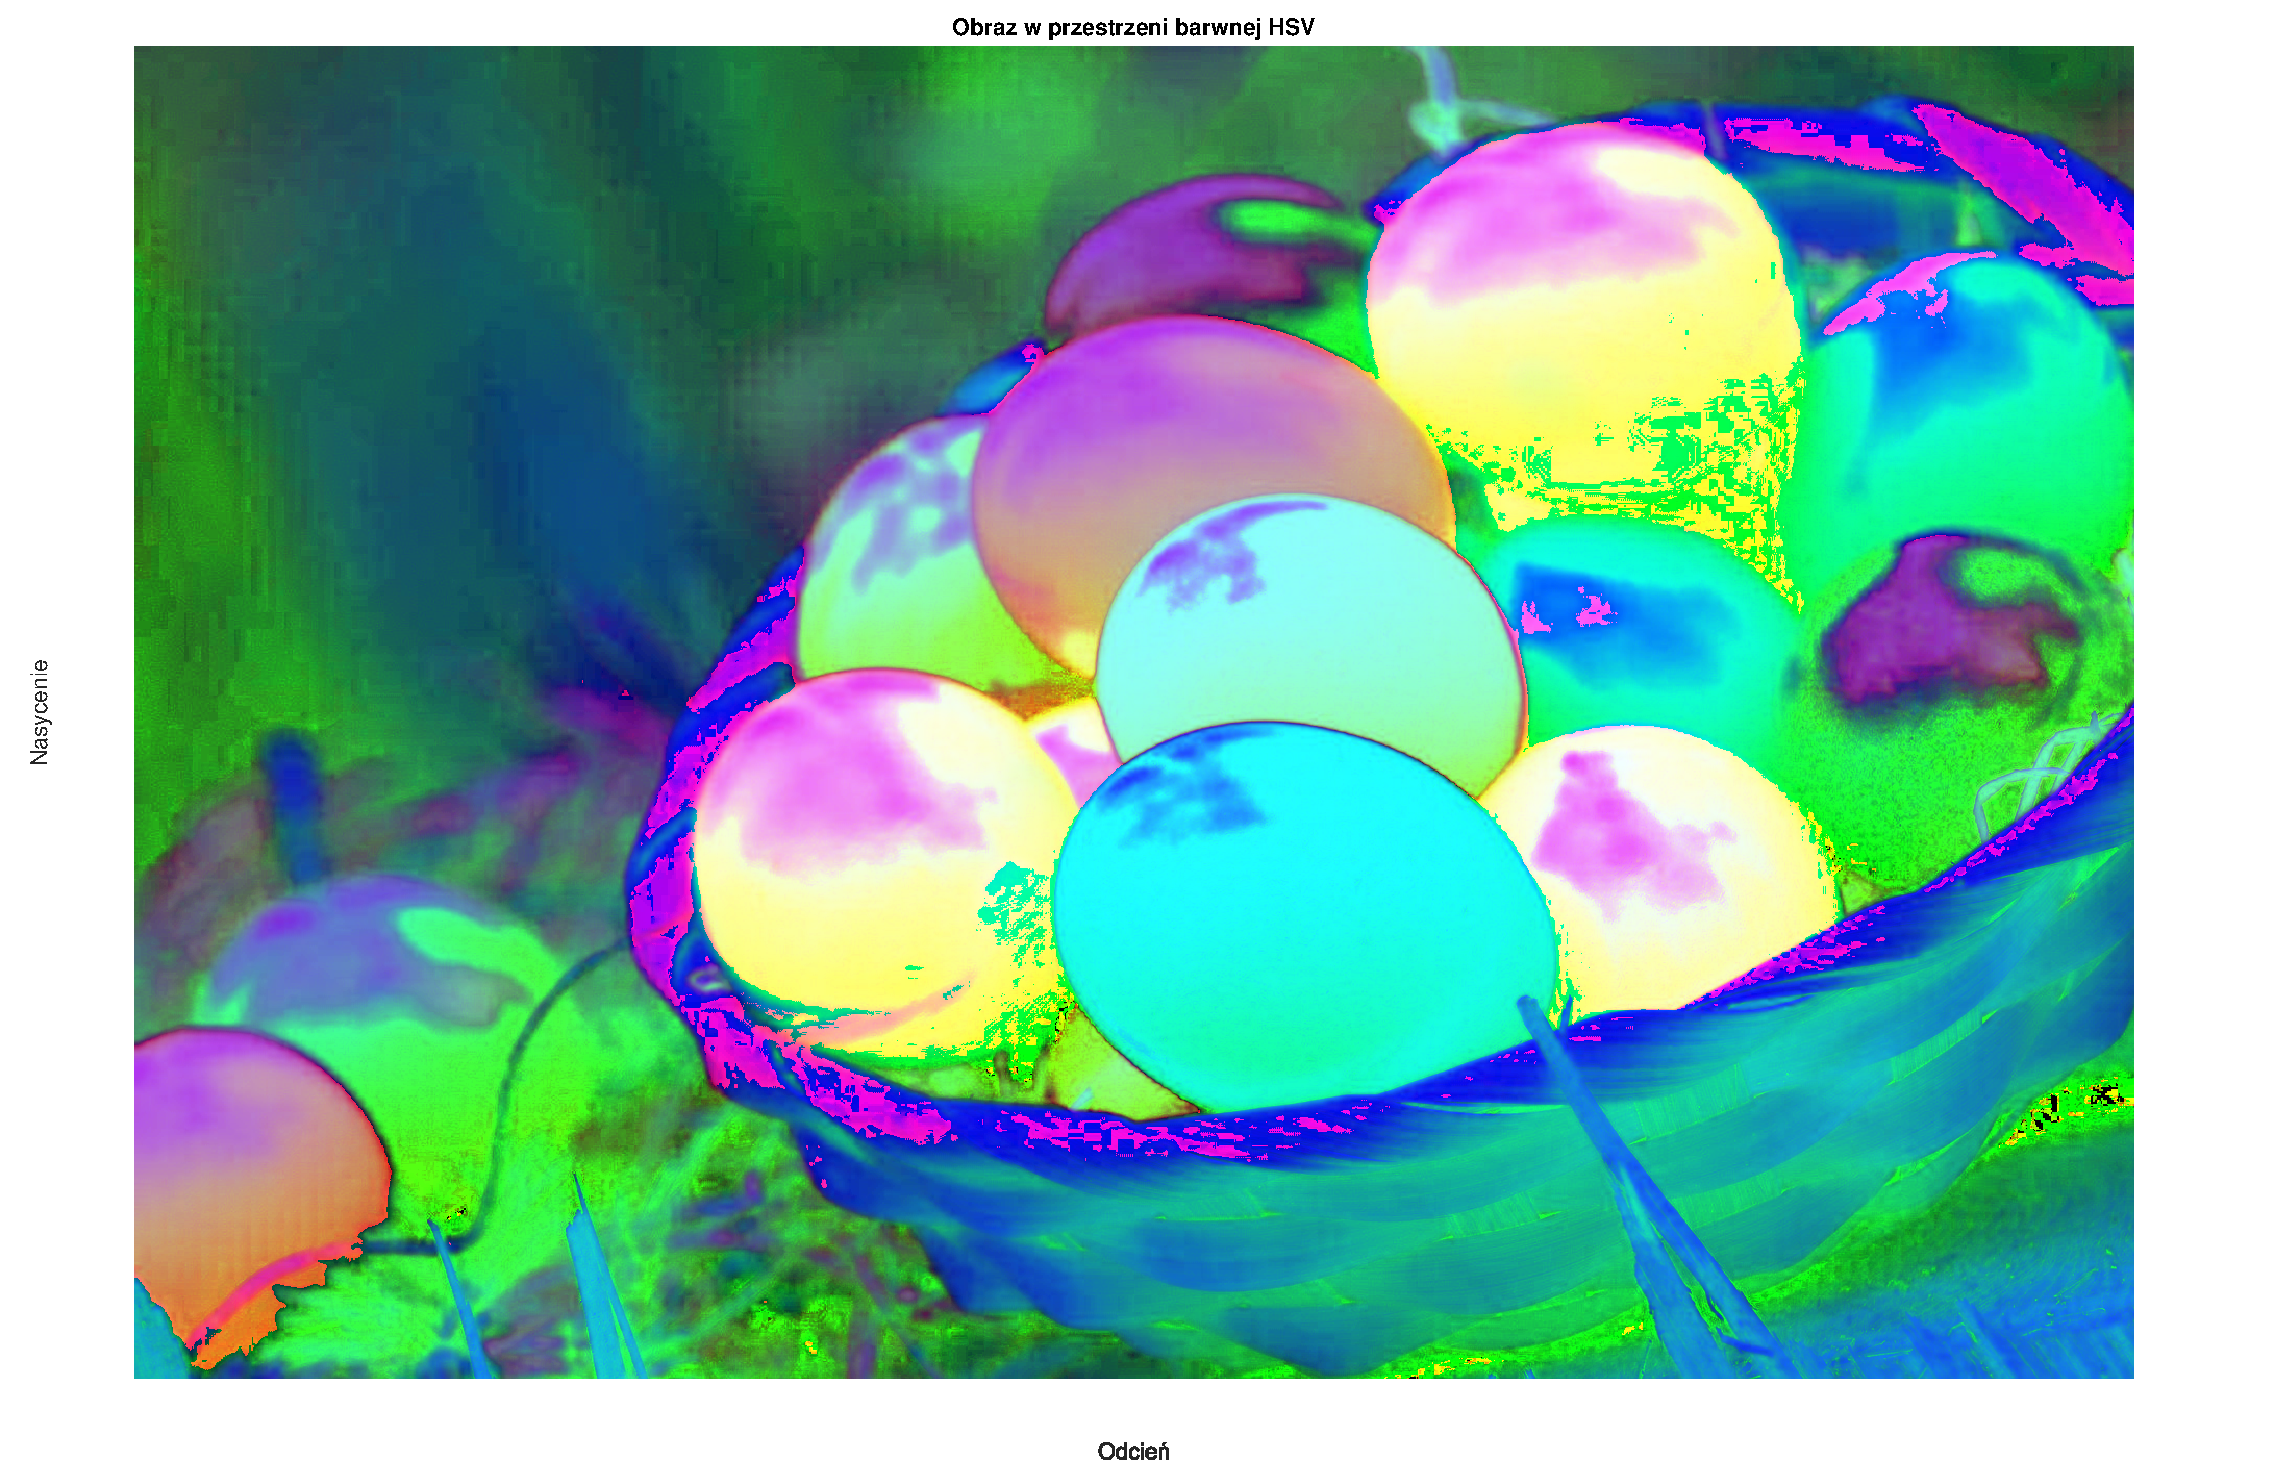
\includegraphics[width=0.9\linewidth]{kod/my_figure6.pdf}\CC\label{fig:my_figure6.pdf}\end{figure}

\begin{figure}[H]\centering\includegraphics[width=0.9\linewidth]{kod/my_figure7.pdf}\CC\label{fig:my_figure7.pdf}\end{figure}

\begin{figure}[H]\centering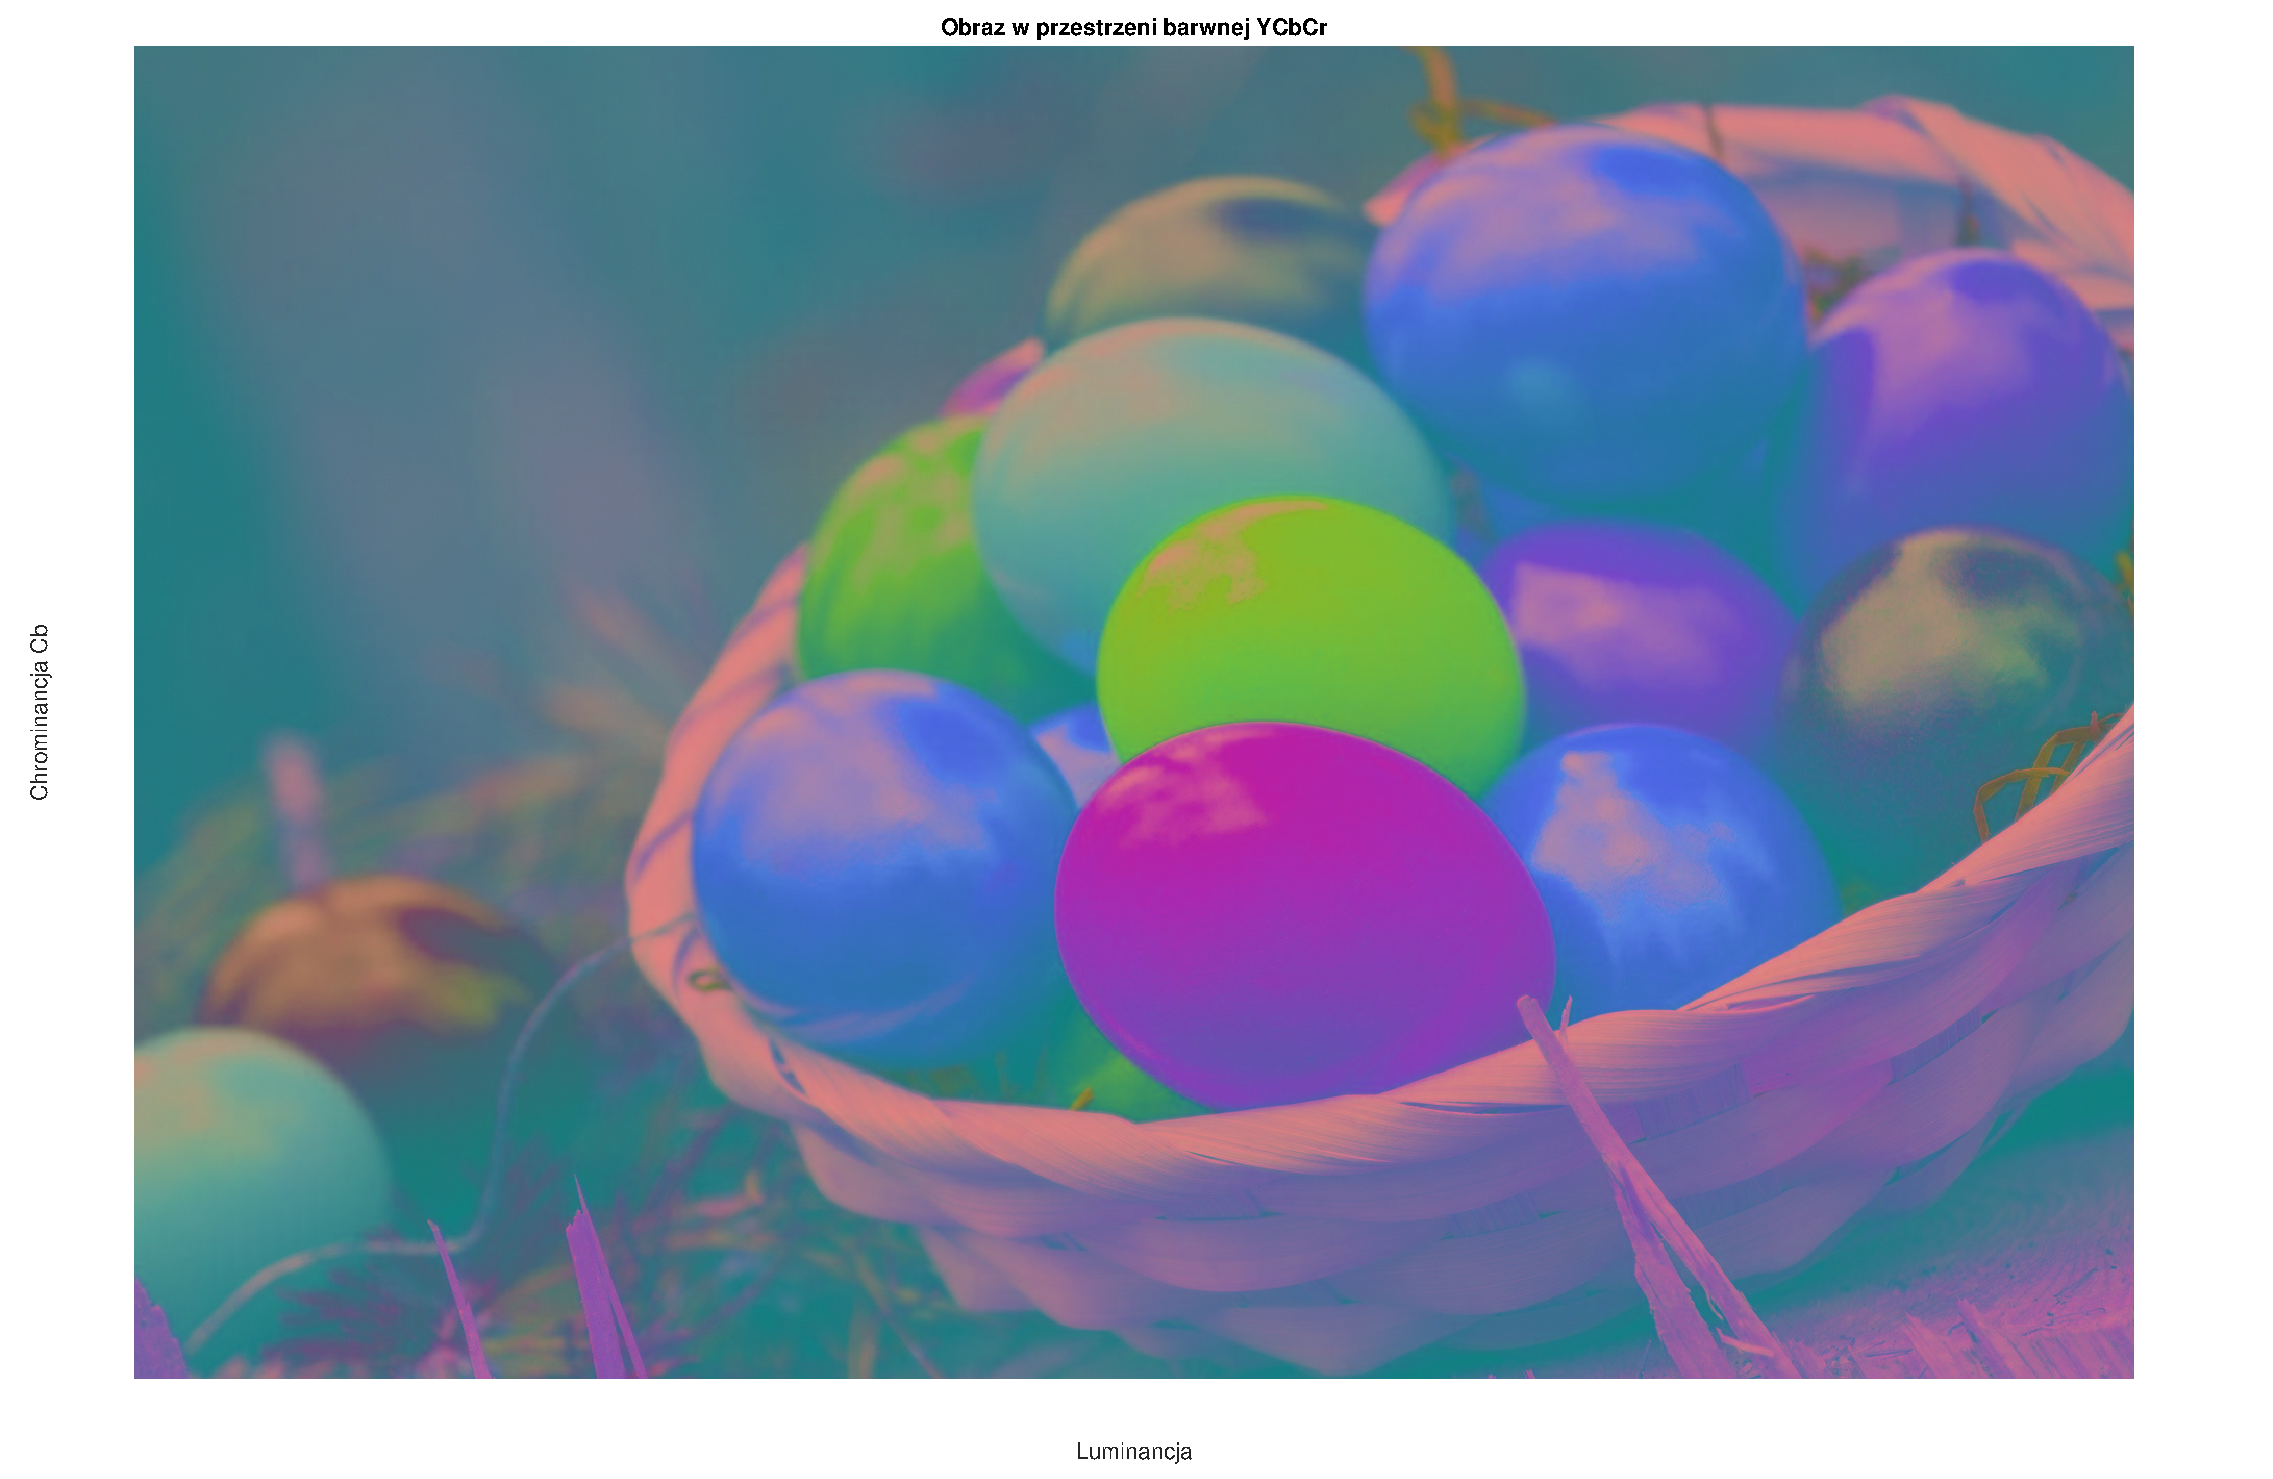
\includegraphics[width=0.9\linewidth]{kod/my_figure8.pdf}\CC\label{fig:my_figure8.pdf}\end{figure}

\begin{figure}[H]\centering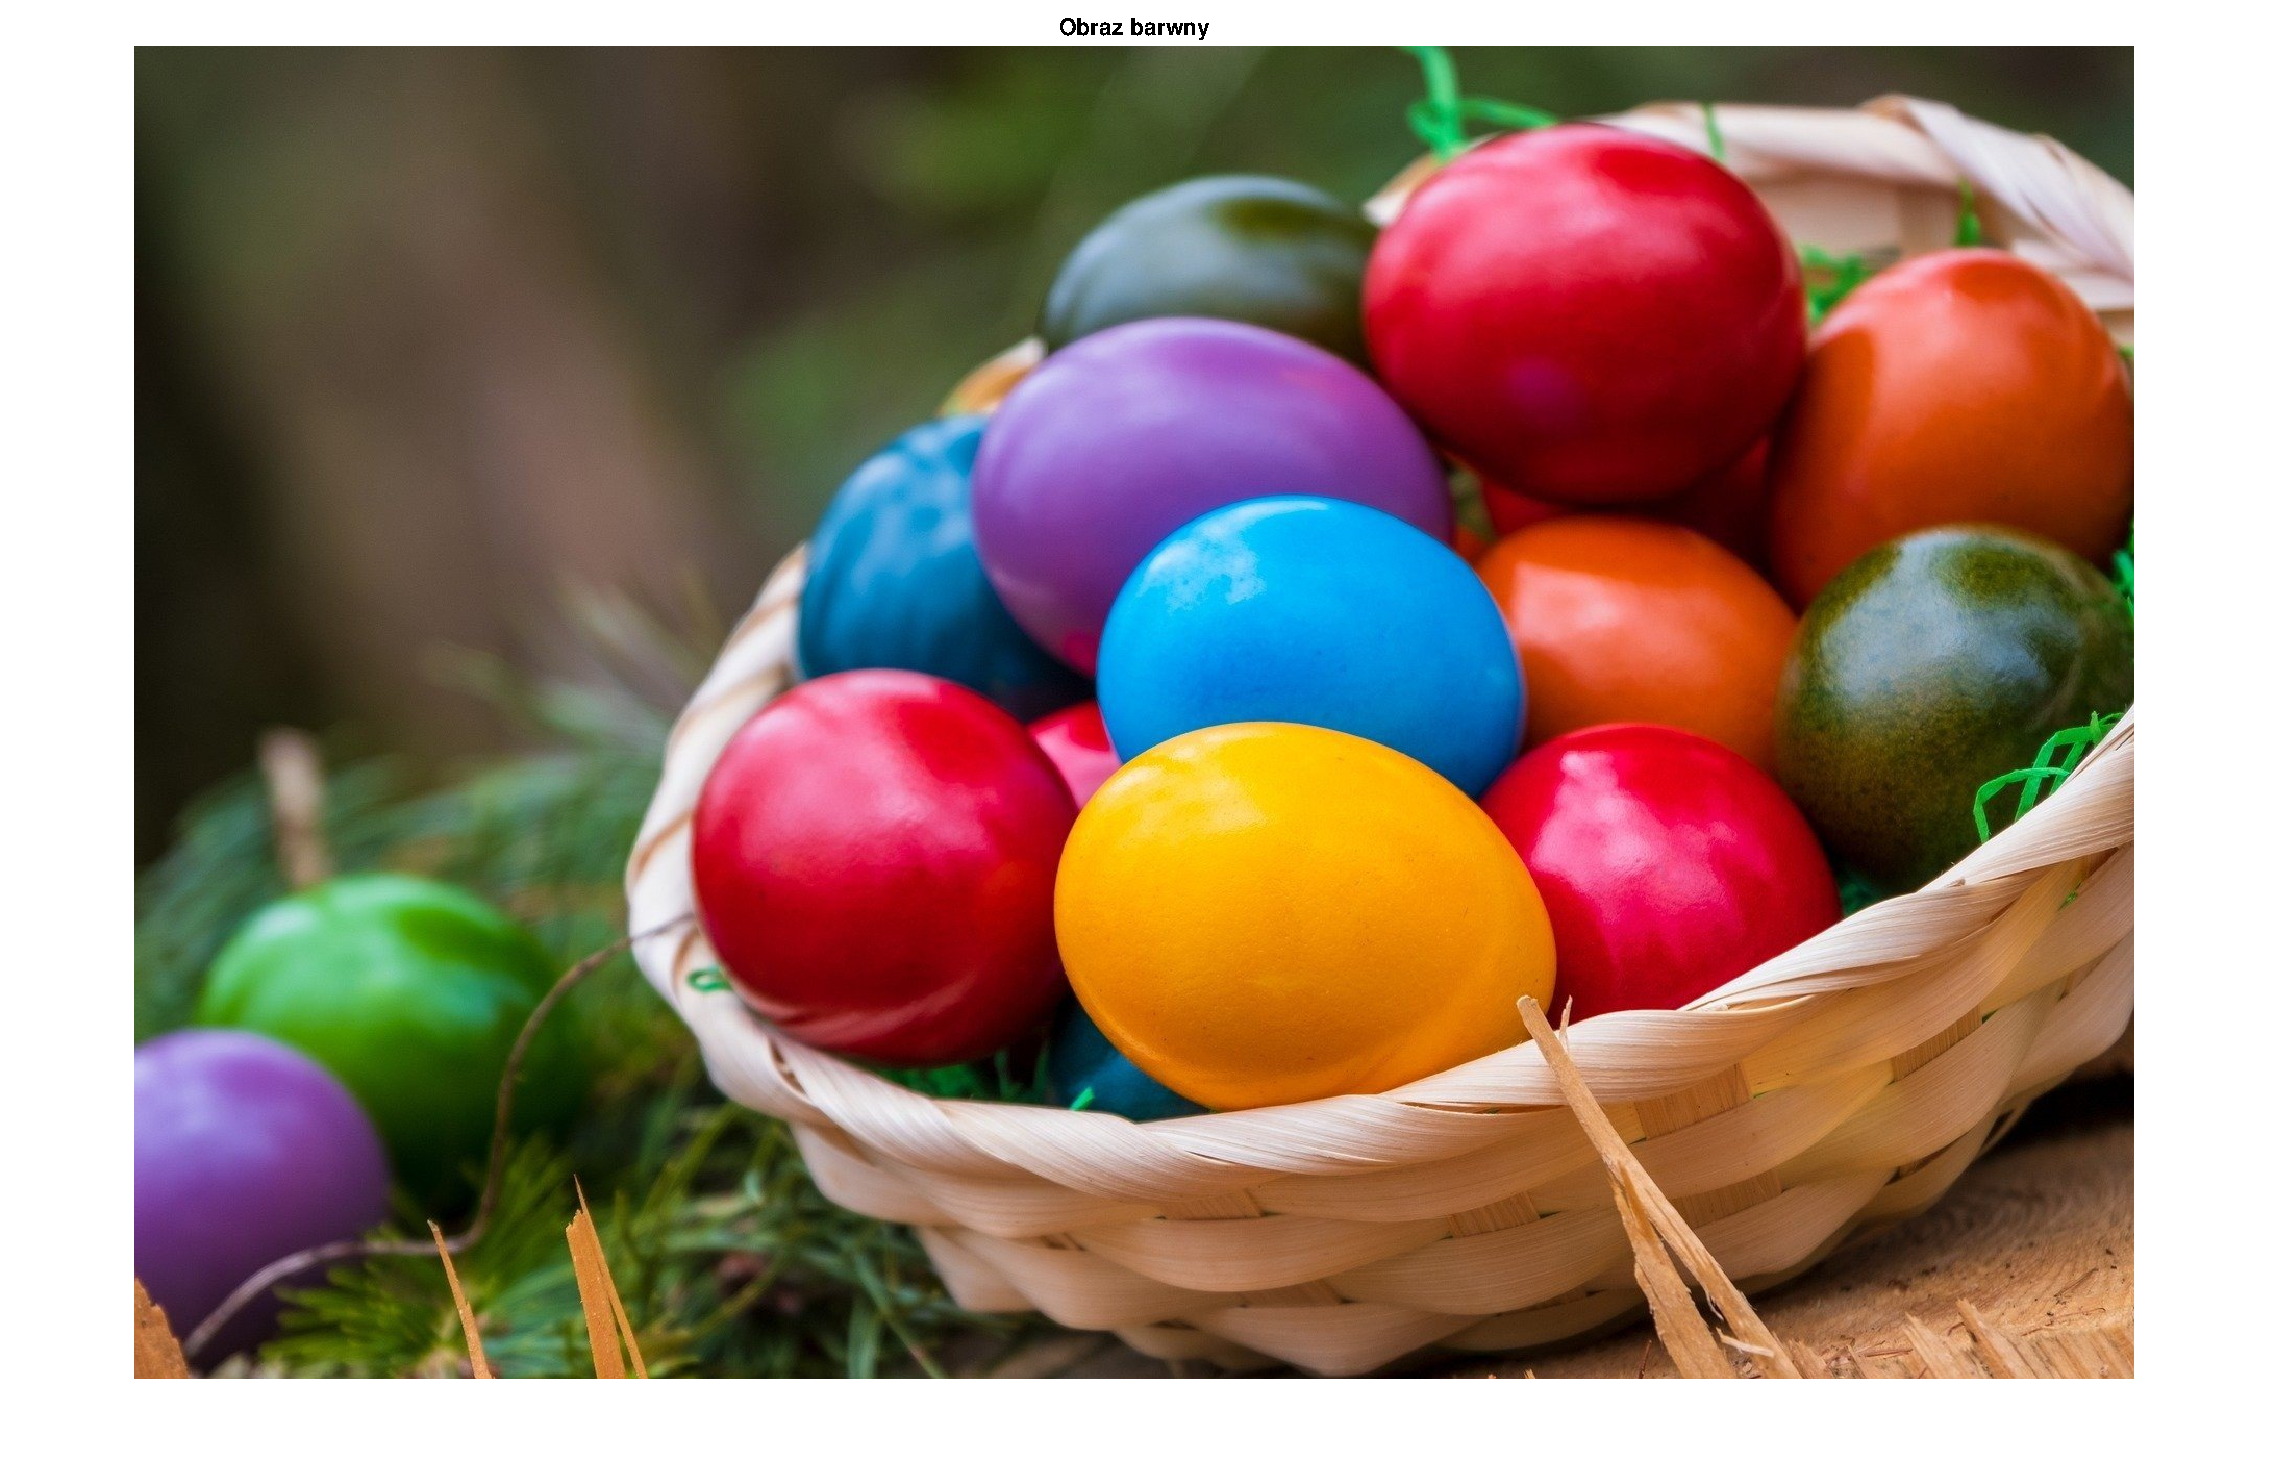
\includegraphics[width=0.9\linewidth]{kod/my_figure9.pdf}\CC\label{fig:my_figure9.pdf}\end{figure}

\begin{figure}[H]\centering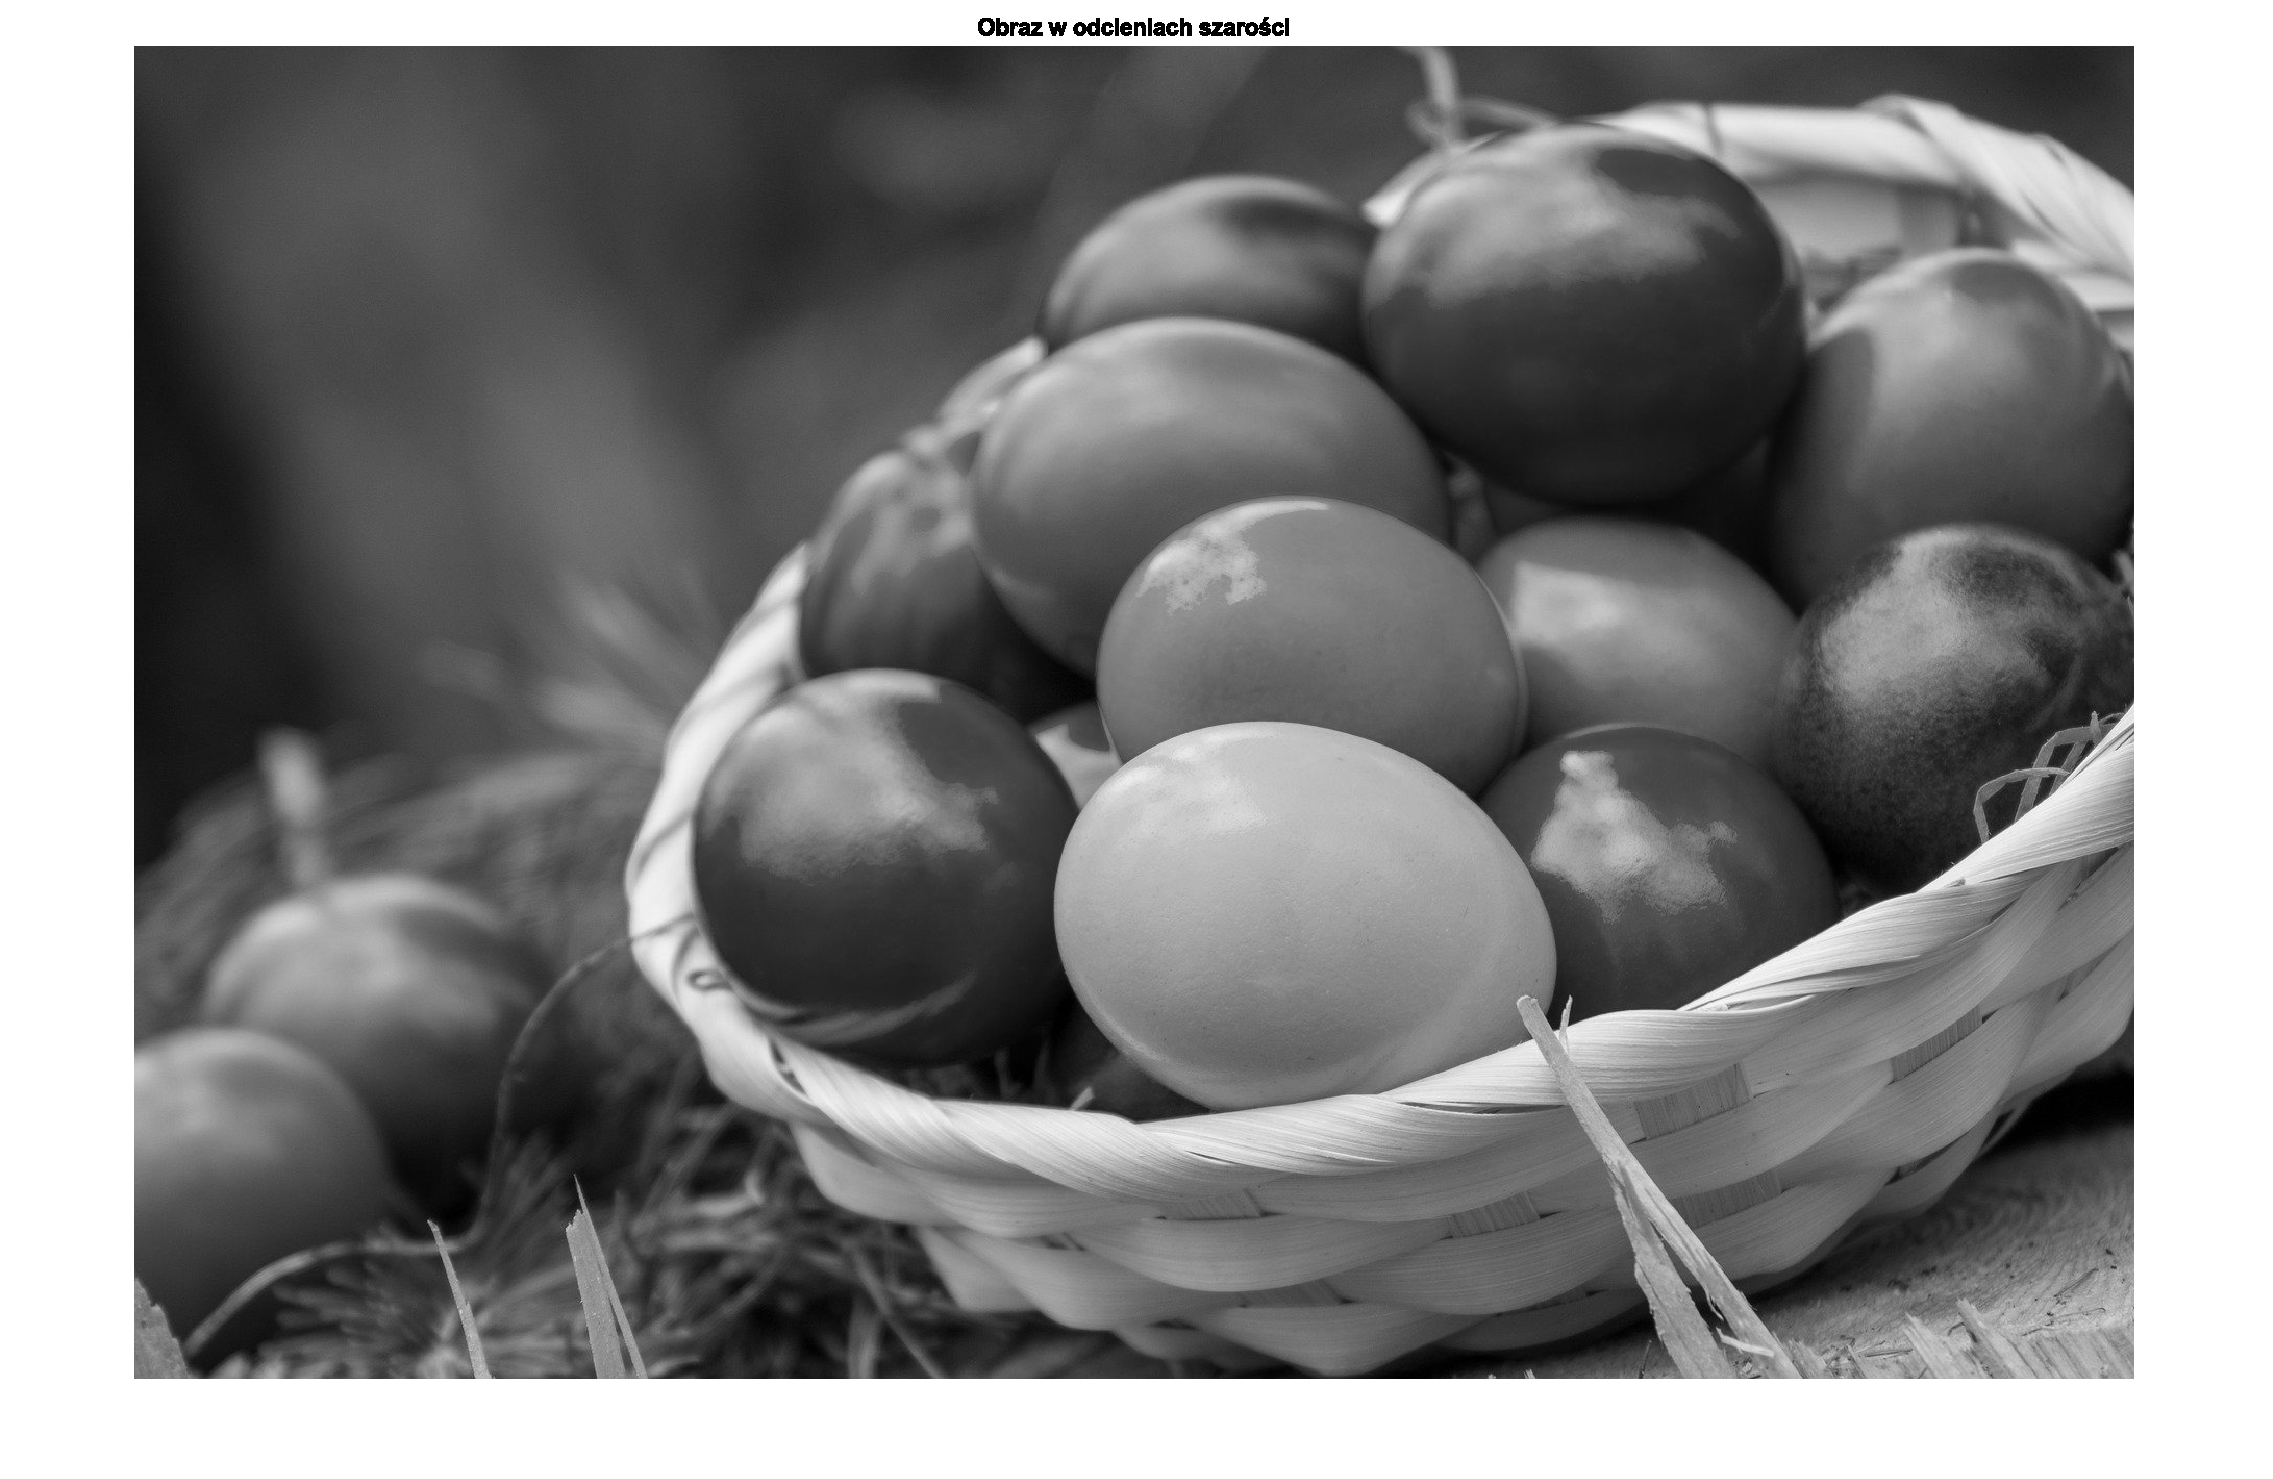
\includegraphics[width=0.9\linewidth]{kod/my_figure10.pdf}\CC\label{fig:my_figure10.pdf}\end{figure}

\begin{figure}[H]\centering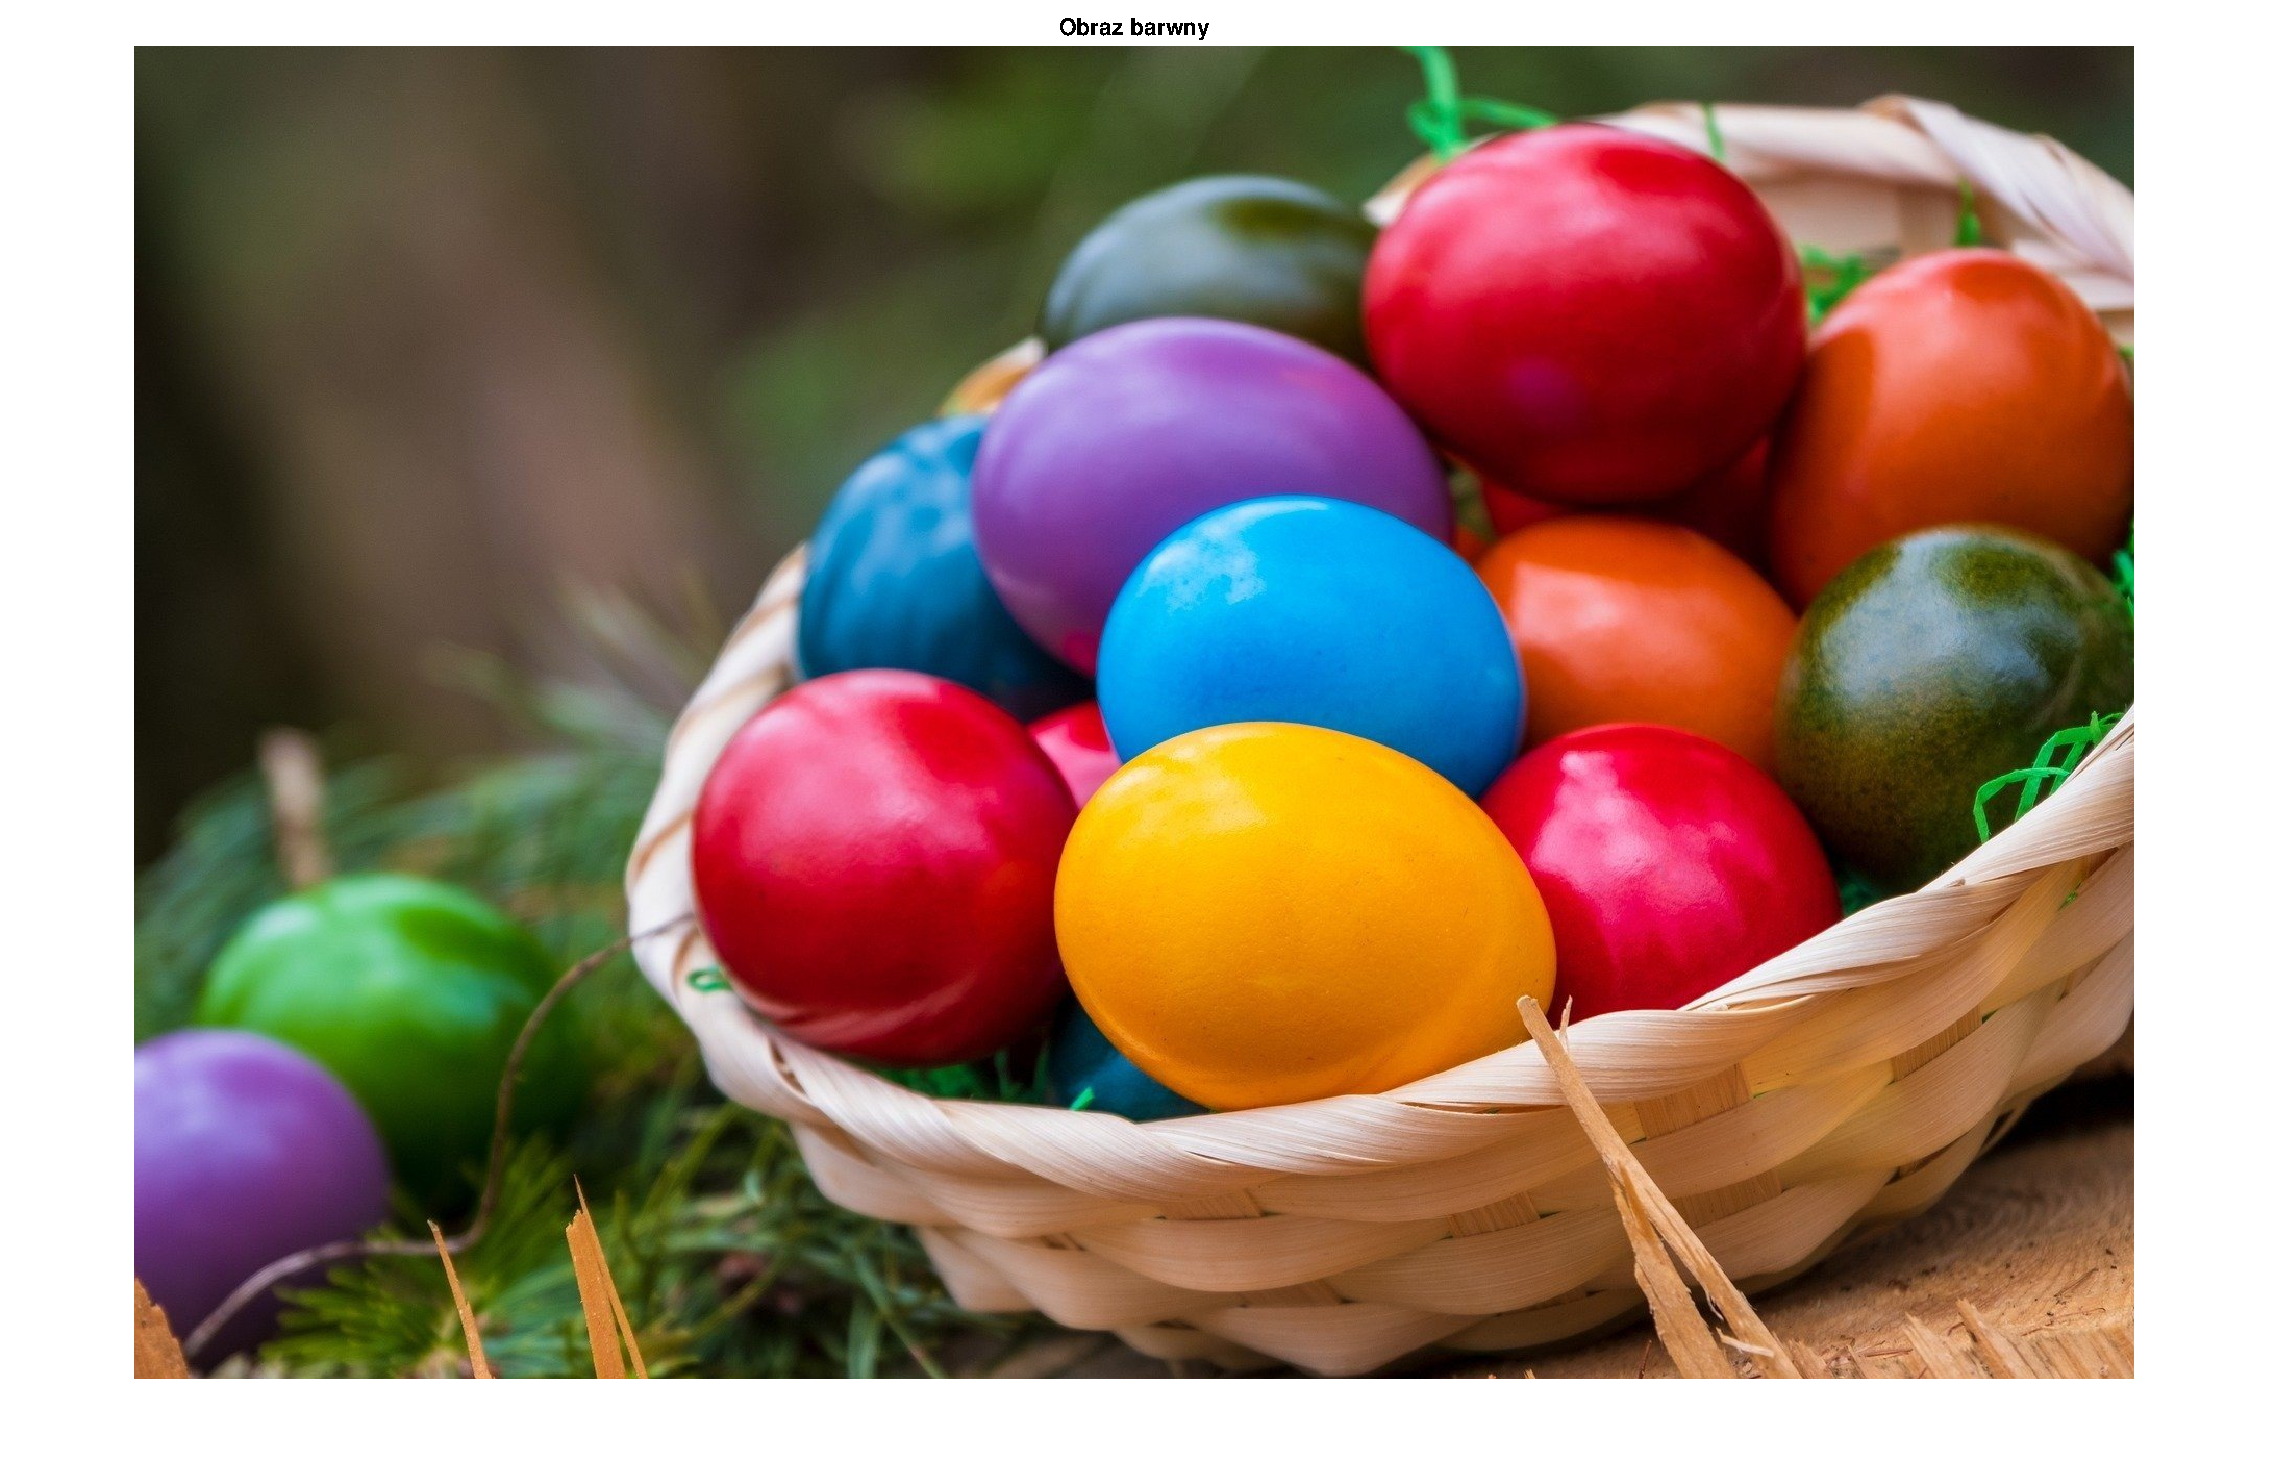
\includegraphics[width=0.9\linewidth]{kod/my_figure11.pdf}\CC\label{fig:my_figure11.pdf}\end{figure}

\begin{figure}[H]\centering\includegraphics[width=0.9\linewidth]{kod/my_figure12.pdf}\CC\label{fig:my_figure12.pdf}\end{figure}

\begin{figure}[H]\centering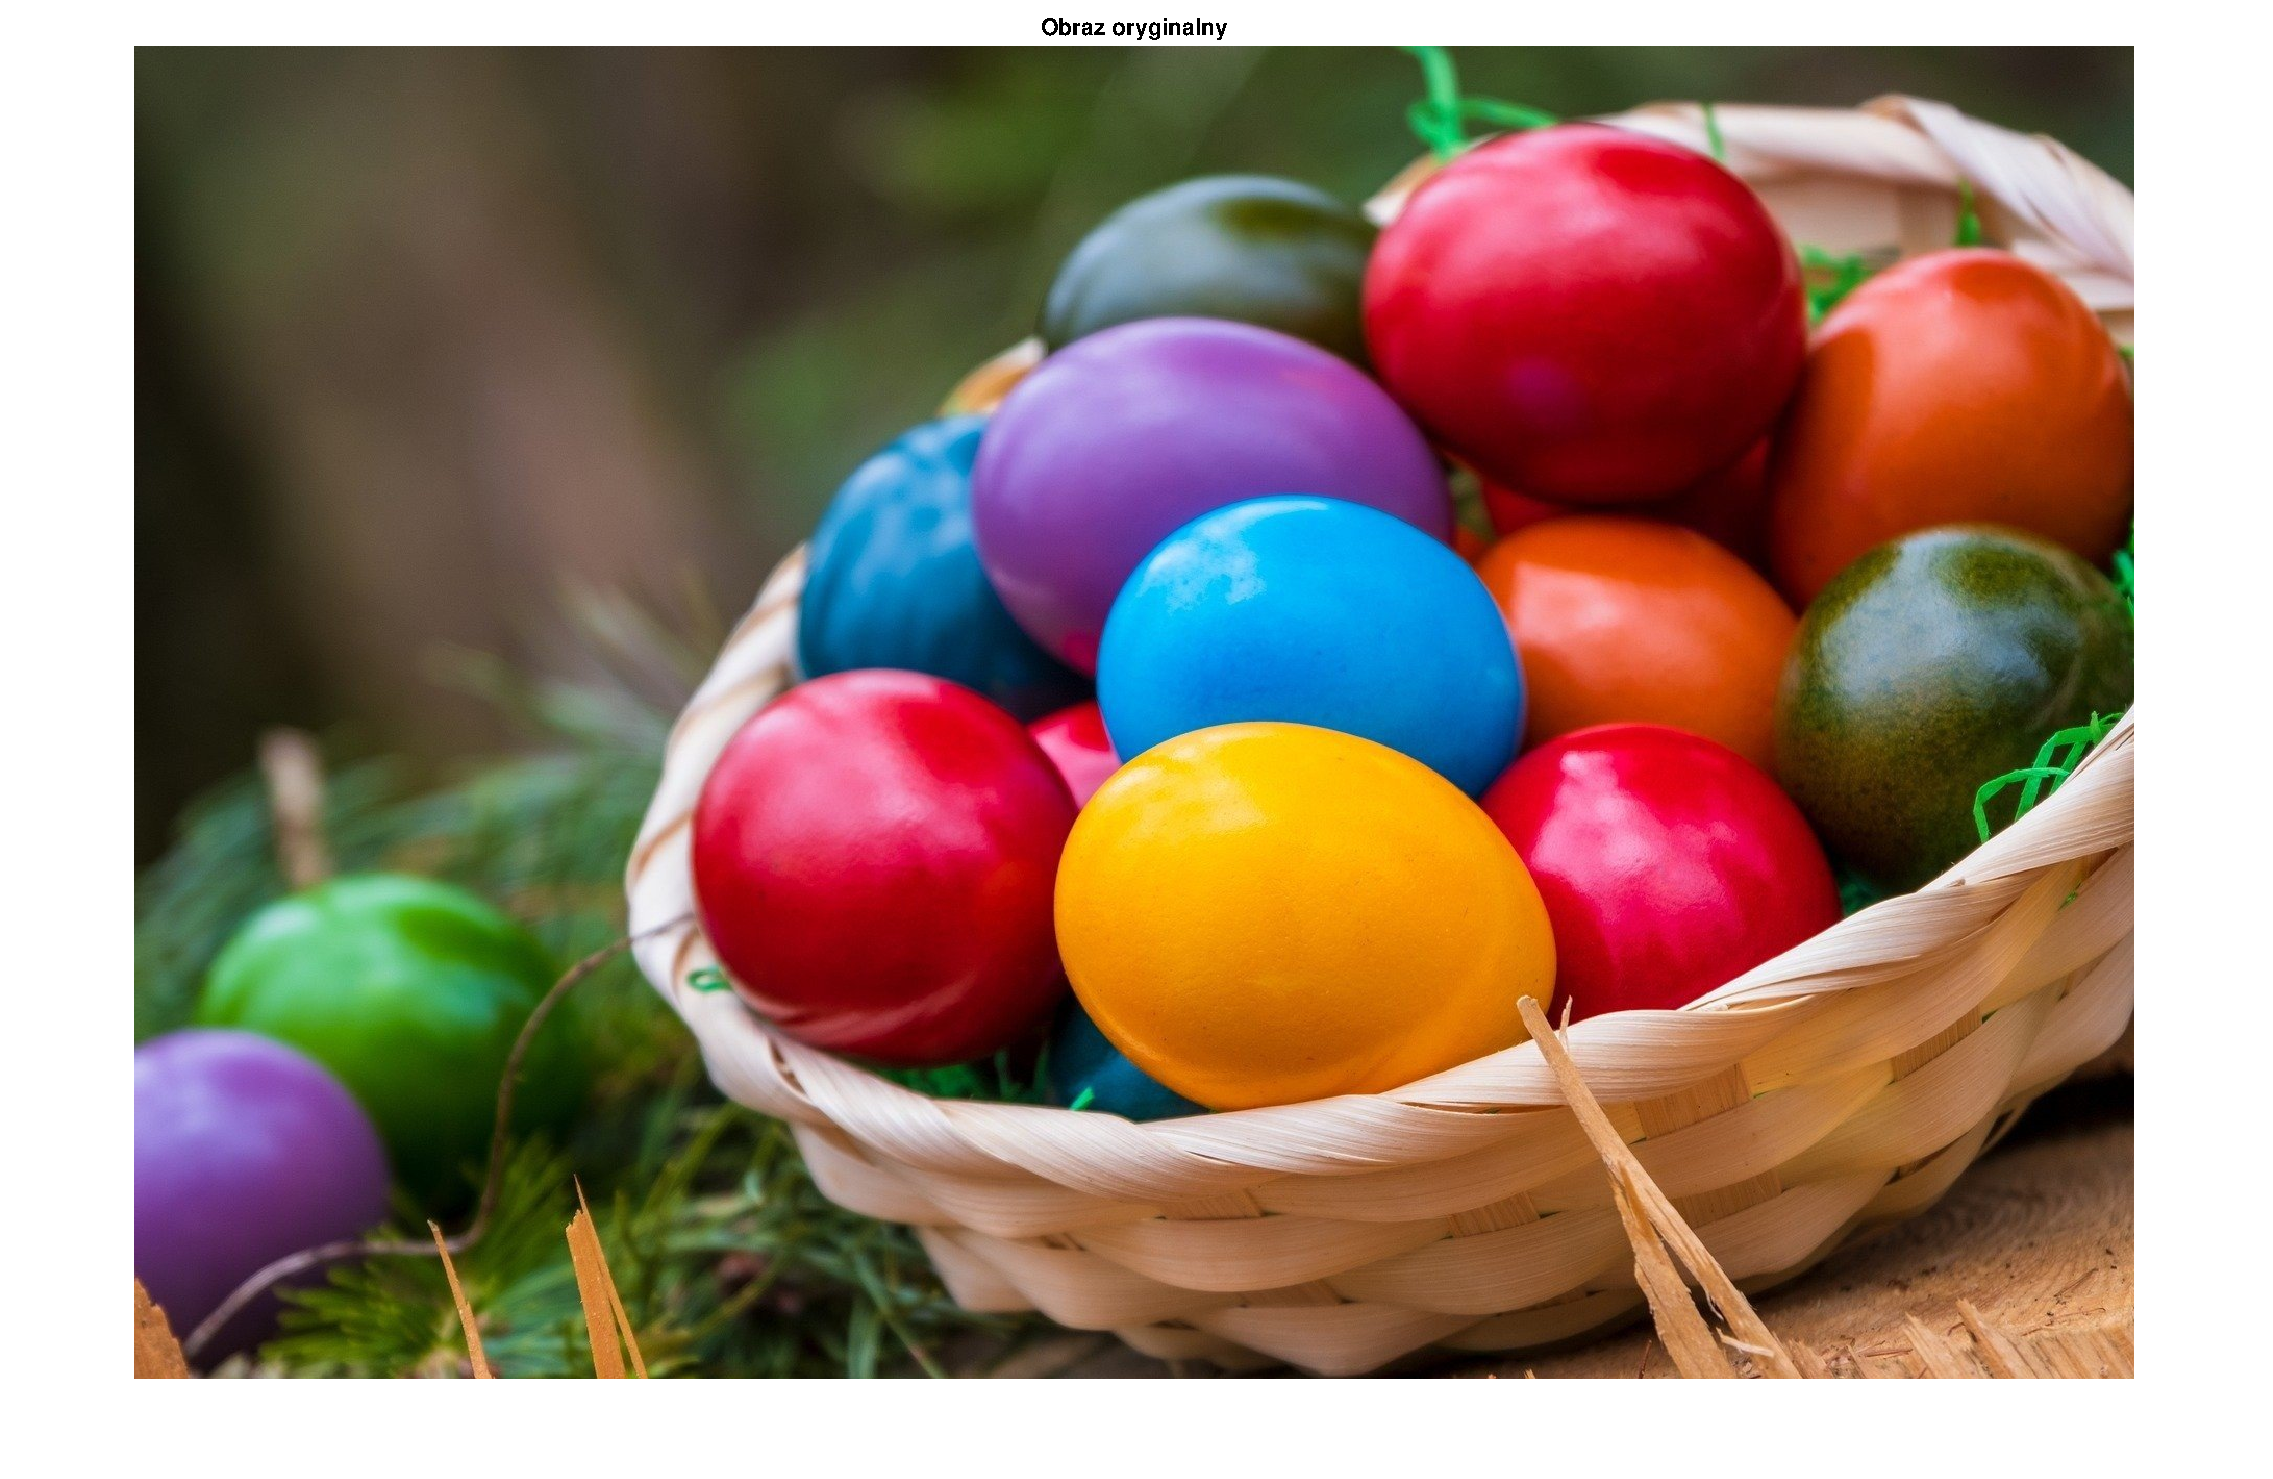
\includegraphics[width=0.9\linewidth]{kod/my_figure13.pdf}\CC\label{fig:my_figure13.pdf}\end{figure}

\begin{figure}[H]\centering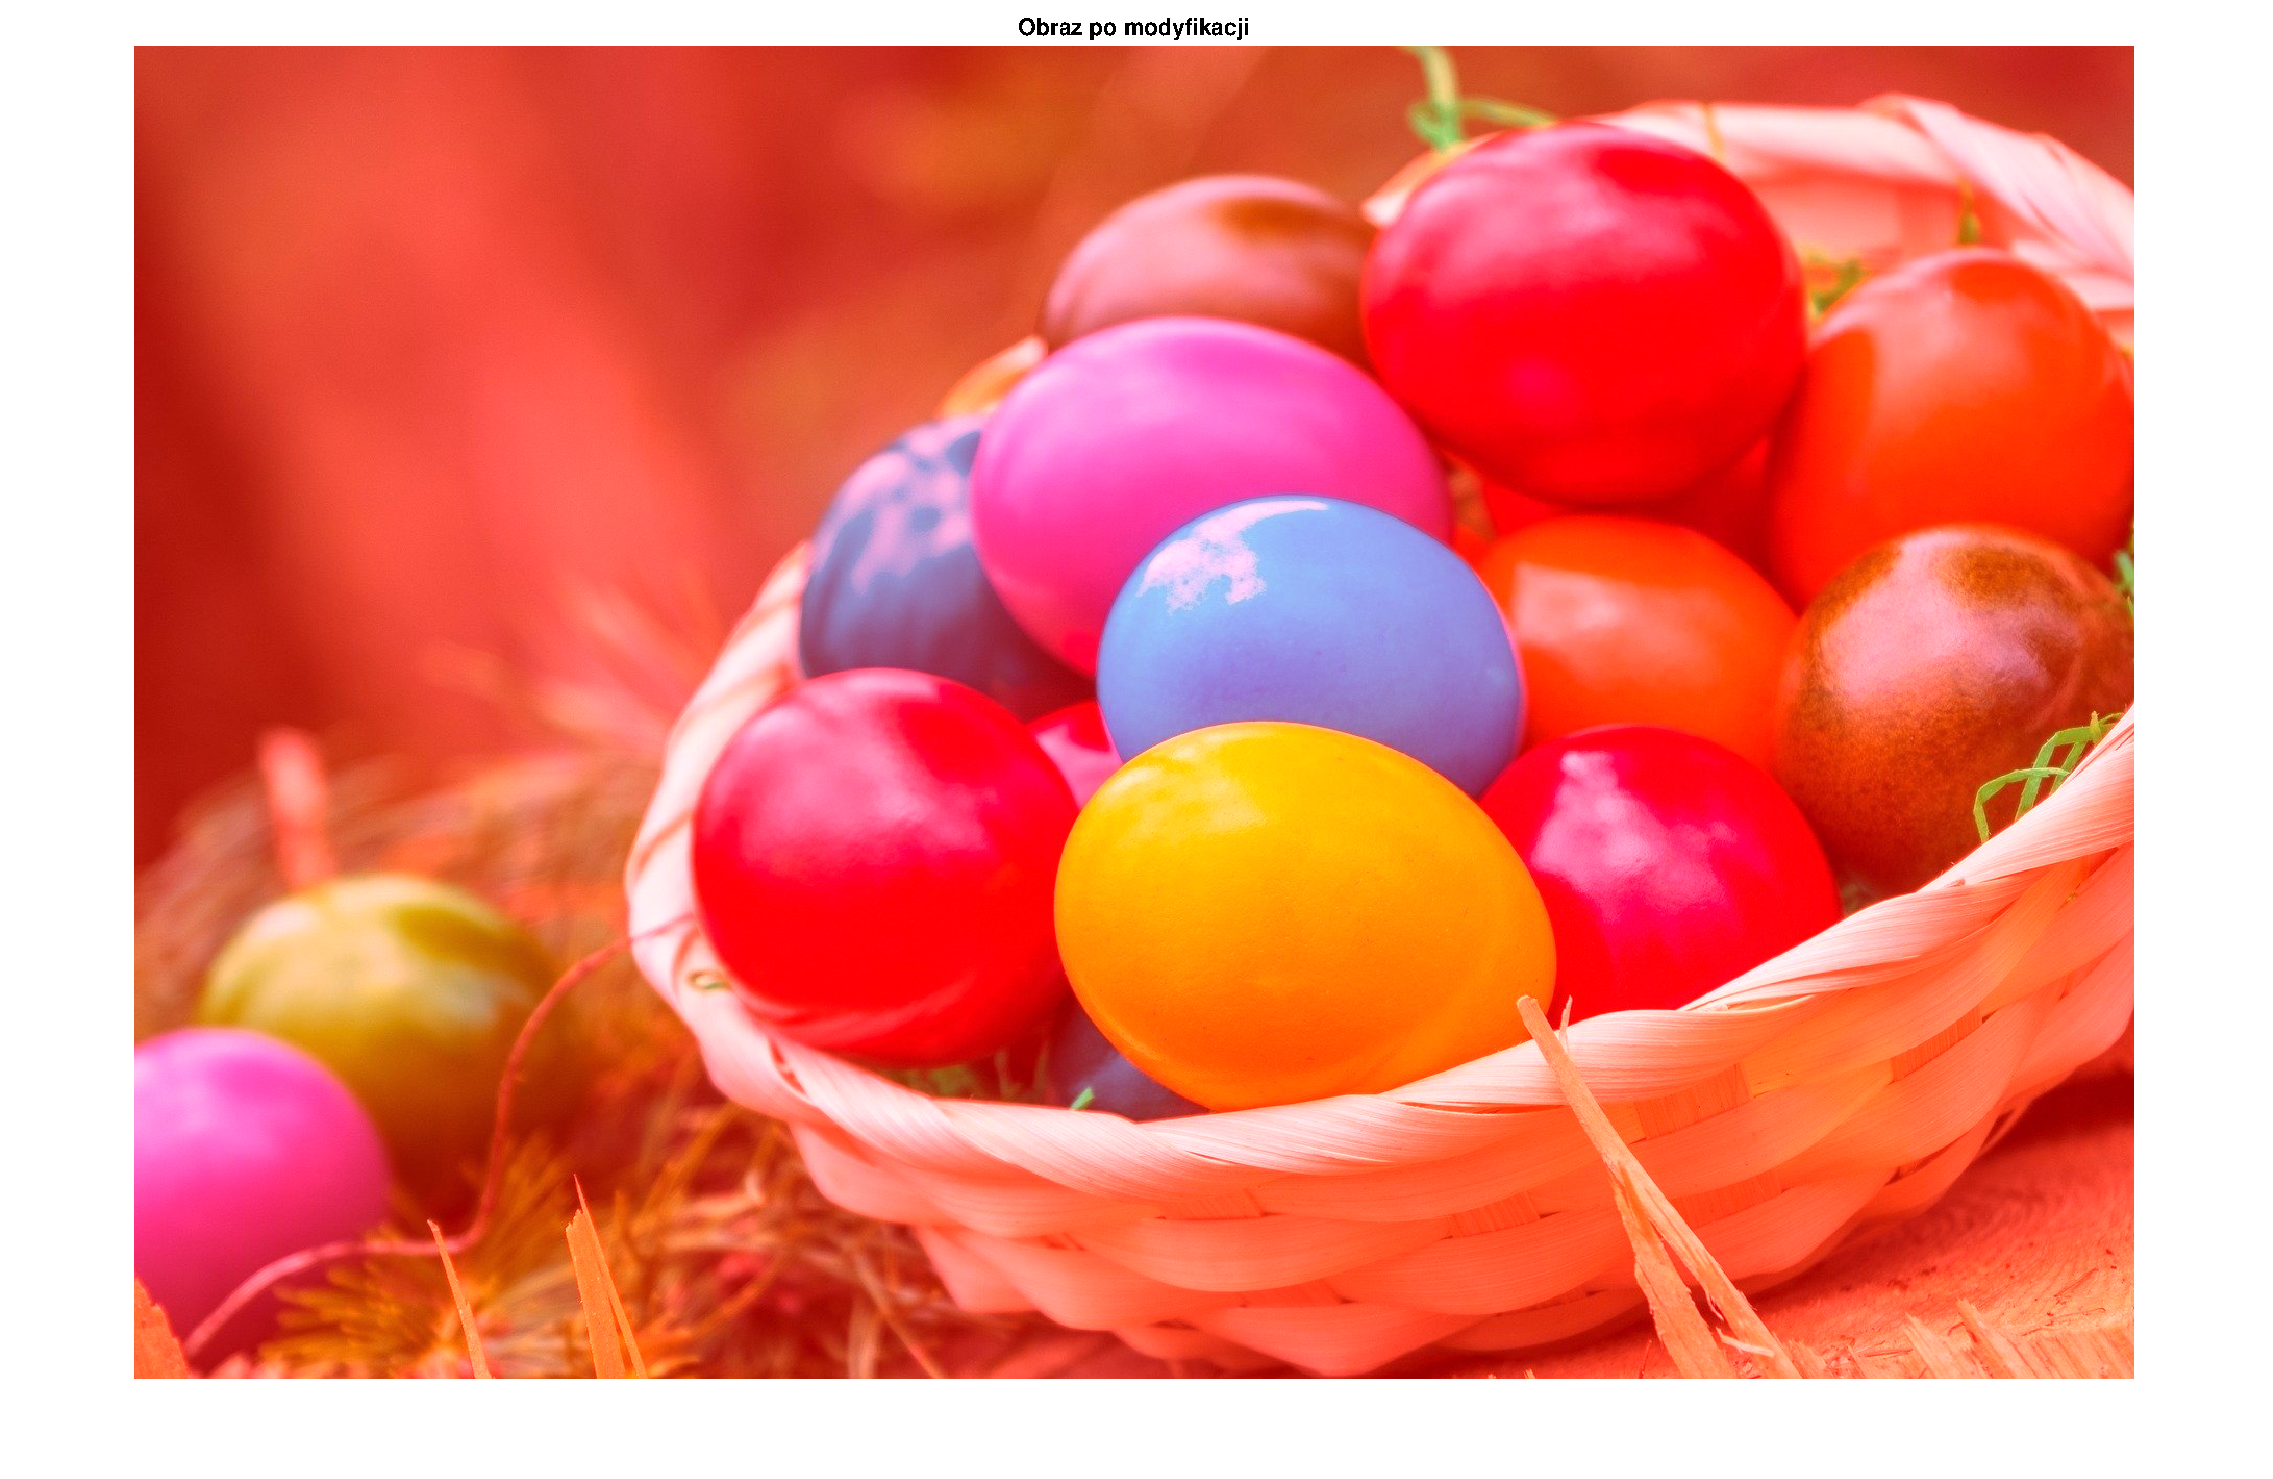
\includegraphics[width=0.9\linewidth]{kod/my_figure14.pdf}\CC\label{fig:my_figure14.pdf}\end{figure}

\begin{figure}[H]\centering\includegraphics[width=0.9\linewidth]{kod/my_figure15.pdf}\CC\label{fig:my_figure15.pdf}\end{figure}

\begin{figure}[H]\centering\includegraphics[width=0.9\linewidth]{kod/my_figure16.pdf}\CC\label{fig:my_figure16.pdf}\end{figure}

\begin{figure}[H]\centering\includegraphics[width=0.9\linewidth]{kod/my_figure17.pdf}\CC\label{fig:my_figure17.pdf}\end{figure}

\begin{figure}[H]\centering\includegraphics[width=0.9\linewidth]{kod/my_figure18.pdf}\CC\label{fig:my_figure18.pdf}\end{figure}

\begin{figure}[H]\centering\includegraphics[width=0.9\linewidth]{kod/my_figure19.pdf}\CC\label{fig:my_figure19.pdf}\end{figure}

\begin{figure}[H]\centering\includegraphics[width=0.9\linewidth]{kod/my_figure20.pdf}\CC\label{fig:my_figure20.pdf}\end{figure}

\section{Wnioski}

Realizacja tego ćwiczenia pozwala studentowi wyciągnąć następujące wnioski dotyczące obróbki obrazów:

\begin{enumerate}
    \item Istnieje wiele przestrzeni barwnych, takich jak HSV, Lab, YCbCr, które oferują różne sposoby reprezentacji kolorów. Przełączanie się między tymi przestrzeniami może być przydatne w różnych zastosowaniach, takich jak analiza, przetwarzanie lub manipulacja obrazem.
    
    \item Konwersja obrazu RGB na odcienie szarości (grayscale) jest jednym ze sposobów redukcji informacji barwnych, pozwalającym skupić się na strukturze i jasności obrazu.
    
    \item Profil barwny RGB dla wybranego obiektu/fragmentu obrazu umożliwia analizę średnich wartości pikseli dla poszczególnych kanałów barwnych. Może być używany do charakterystyki barwy danego obiektu i porównywania go z innymi obiektami.
    
    \item Modyfikacja kanałów barwnych, takich jak dodawanie, odejmowanie, mnożenie itp., pozwala na manipulację kolorami obrazu i uzyskanie różnych efektów wizualnych.
    
    \item Pseudokolorowanie obrazów pozwala na przypisanie kolorów do wartości odcieni szarości, co może ułatwić percepcję różnic w intensywnościach pikseli.
    
    \item Wyodrębnianie określonych kolorów na obrazie może być użyteczne w analizie obrazów i wyodrębnianiu obiektów o konkretnych cechach barwnych.
    
    \item Regulacja kontrastu obrazu może poprawić jego jakość wizualną i uwypuklić szczegóły w obrazie. Różne wartości parametrów regulacji kontrastu mogą prowadzić do różnych efektów wizualnych.
    
    \item Pomiar różnicy kolorów z wykorzystaniem funkcji deltaE i imcolordiff pozwala na analizę różnic pomiędzy dwoma obrazami lub ich fragmentami. Może być przydatne w analizie kolorystycznej, porównywaniu obrazów lub identyfikacji różnic między nimi.
\end{enumerate}

Ogólnie rzecz biorąc, to ćwiczenie pozwala studentowi na zdobycie praktycznego doświadczenia w obróbce obrazów, eksploracji różnych przestrzeni barwnych, regulacji kontrastu, wyodrębnianiu kolorów i analizie różnic kolorystycznych. Jest to cenne w zrozumieniu podstawowych technik przetwarzania obrazów i ich zastosowań w różnych dziedzinach.

\end{document}
